\chapter{Is market power in Australia stronger than elsewhere?\label{chap:international}}

Australia is often said to be an economy dominated by duopolies and oligopolies.%
    \footcite{Macrobusiness_duopoly_2017}
And there is concern that Australia has more highly concentrated industries than other countries.%
    \footcite{Ritter-Guardian-2013}

\begin{quote}
    `In every sector of the Australian economy we have an effective duopoly or oligopoly at work.'

    \rightline{-- \textcite{Macrobusiness_oligopoly}}
\end{quote}

\begin{quote}
    `Girt by sea, Australia has proved a breeding ground for monopolies, or oligopolies \dots It's hard to turn around without seeing the corporate logo of some oligopolist. No wonder we Australians so often feel like we're getting ripped off, either paying more than we should in a truly competitive market or simply not getting the service that we deserve.'

    \rightline{-- Jessica \textcite{Irvine_oligopolies_2011}}
\end{quote}     

This chapter compares the market shares of large firms in some large concentrated sectors in Australia to those in other economies. It finds that many of those sectors are concentrated elsewhere, but the supermarket sector is unusually concentrated in Australia. 

\section{Australia's economy is concentrated, but not unusually so \label{sec:int_comp}}

Most large concentrated sectors are not more concentrated in Australia than they are in other high-income economies of a similar size. \Vref{fig:cross_concentration} compares concentration in the largest highly concentrated sectors in Australia by revenue: banking, supermarkets, mobile telecommunications, internet service provision, fuel wholesale and retail, and general, life and health insurance.\footnote{These sectors are in the `scale-economies' or `higher-regulation' sector groups. Comparisons of natural-monopoly sectors are excluded, because they are uniformly highly concentrated, at the local level.}

% The similarity of concentration levels between sectors indicates there are common barriers to entry in every country. However, the fact that Australia has similarly concentrated sectors to other high-income countries does not mean concentration is not a problem. It is possible many countries struggle to increase competitive pressure in their markets.%However concentration could also be a symptom of economies of scale, well managed natural monopoly assets and deliberate regulation in modern industrial economies. \Chapref{chap:profits} investigates the profits, the other indicator of market power, in these sectors.

\begin{figure}
   \caption{Most of Australia’s large, scale-economy sectors are not unusually concentrated \label{fig:cross_concentration}}
    \units{Concentration ratios by sector, per cent}
    \includegraphics[page=7]{atlas/Charts} 
    \noteswithsources{Bubbles typically represent OECD economies or large US state economies. Bubble size represents population. a: 3-firm; b: 4-firm; c: 5-firm. Unshaded bubbles mean that fewer firms are represented.
    %Supermarkets 4-firm except Italy, Florida, Netherlands and Portugal 3-firm market share. Health insurance 5-firm, except Florida and Texas 3-firm market shares. Australia's fifth largest life insurer has less than 5 per cent market share and is not included. Fuel wholesale 4-firm except Greece (2-firm), and Turkey and Bulgaria (1-firm). Fuel retail 5-firm except Chile, Portugal, Turkey and Germany 4-firm market share, and Spain and Bulgaria 3-firm market share.\\
    }{See \Cref{fig:banks_OECD}, \Cref{fig:supermarkets}, \Cref{fig:mobile}, \Cref{fig:ISPs}, \Cref{fig:health}, \Cref{fig:Insurance}, and \Cref{fig:Fuel}.}
\end{figure}

These sectors are quite highly concentrated in most high-income economies. They also tend to be less concentrated in large economies than in small ones, when measured at the national level. Concentration in most of these large sectors is not much different in Australia than other economies:%
%\footnote{Concentration levels vary between countries due tax and regulations that favour larger or smaller businesses, regional concentration differences, proximity of trading partners, free trade unions and agreements, and population size and distribution.}
\begin{itemize}
\item \textbf{Banking:} the three-firm market share in Australia is about 70 per cent, which is in the middle of the range for high-income economies. The five-firm share is at the high end of the range for economies of a comparable size. 
\item \textbf{Supermarkets:} the four-firm market share in Australia is around 90 per cent. This is high compared to other high-income countries.
\item \textbf{Mobile telecommunications:} the three-firm market share in Australia is 100 per cent. High-income countries tend to have only three or four networks, and their three-firm market shares typically exceed 80 per cent.
\item \textbf{Internet service providers} (ISPs): the four-firm market share in Australia is 89 per cent. This is similar to France, the UK and the Netherlands, but much higher than the US, Japan and Canada, where the combined market share of the four-largest ISPs is about 60 per cent.\newpage
\item \textbf{Fuel wholesale and retail:} in Australia the four-firm fuel wholesaling market share is 91 per cent, and the five-firm fuel retailing market share is 72 per cent. Neither differs much from the market shares in other high-income economies.
\item \textbf{General insurance:} the five-firm market share in Australia is almost 90 per cent. This is high compared to most other high-income economies, which range from 25 per cent to 81 per cent.
\item \textbf {Life insurance:} the four-firm market share in Australia is 44 per cent. This is low compared to other high-income economies, which range from about 40 per cent to almost 100 per cent.
\item \textbf{Health insurance:} the five-firm market share in Australia is 78 per cent. This is slightly lower than other similar-sized countries, such as the Netherlands, and US states, such as Texas, but much higher than the US as a whole, and Germany.
\end{itemize}

% These sectors are typically highly concentrated in all high-income economies for which data is available.%
% \footnote{Largest firms are either the largest 3, 4 or 5 firms as noted on \Cref{fig:cross_concentration}. 
% For details see notes included on individual sector charts.} 

% But concentration within a state or region of a large economy can be much higher.

The following sections cover in more detail three of the largest concentrated sectors with barriers to entry: banks, supermarkets, and mobile telecoms.

\clearpage

\subsection{Banking in Australia is about as concentrated as it is in other economies of similar size}

\begin{figure}
   \caption{Banking in Australia is not unusually concentrated \label{fig:banks_OECD}}
    \units{Three-firm banking concentration, OECD economies, per cent}
    \includegraphics[page=8]{atlas/Charts} 
    \notewithsource{Assets of three largest banks as a share of assets of all commercial banks, 2007-2011 average}{Grattan analysis of \textcites{WorldBank-GFDD-2017}{oecd.stat}.
    }
\end{figure}

Competition in banking is of concern to many Australians. While the Murray Financial System Inquiry concluded that `on balance, the banking sector is competitive', it recommended that competition across the financial system be monitored. The Government has recently asked the Productivity Commission to review competition in the financial system, including in investment, business and personal banking.%
    \footcites{PC-FScompetition-2017,FSI-2014}
The ACCC's view, by contrast, is that `the current oligopoly structure is not vigorously competitive and has not been for some time'.
\footcite{ACCC-PC-submission}

Banking in Australia is not much more concentrated than it is in other high-income economies of about the same size. The market share of the biggest 3 banks is about 70 per cent. That share exceeds 60 per cent in more than two-thirds of OECD countries (\Vref{fig:banks_OECD}). The market share of the biggest 5 banks is a bit higher than other economies about Australia's size (\Vref{fig:5banks}) %

    % \footnote{In Australia, financial services are 8-to-10 per cent of value-added, and in the European Union the average is around 5 per cent; \textcite{OECD-VA-2017}.}

The Reserve Bank of Australia recently concluded that `[t]he concentration of the banking system in Australia is not unique internationally but it is at the high end'.%
\footcite{BullockBigBanks2017}

The banking sector in economies larger than Australia, such as the US, the UK, France and Japan, tend to be less concentrated, when measured at the national level. Low concentration at the national level in the US is in part the legacy of regulations that once limited multi-state banking. %
%Concentration at the national level in the US increased in recent decades as banks merged after these multi-state banking restrictions were relaxed. 
Banking market concentration in the US is much higher when measured at the state level.%
    \footcites{FDIC-bank-US, Neely-1994, Sherter-CBS-2009}

%Competition in banking is a function of much more than just aggregate concentration ratios, of course.

\clearpage
\subsection{Supermarket retailing in Australia is relatively concentrated}

\begin{figure}
    \caption{Supermarket retailing in Australia is concentrated \label{fig:supermarkets}}
    \units{Top four-firm market shares by revenue, per cent}
  \includegraphics[page=9]{atlas/Charts} 
  \notewithsource{Sorted by population. Fourth firm data unavailable for Italy, Florida, the Netherlands, and Portugal.}{Grattan analysis of \textcites{Statista_grocery_Ireland}{Loof_grocery_Sweden}{Statista_grocery_Portugal}{Gain-grocery-Benelux}{DN-grocery-Netherlands}{RoyMorgan-grocery-Australia}{UFCW-grocery-Canada}{Statista_grocery_Spain}{Statista_grocery_Italy}{Statista_grocery_France}{Statista_grocery_UK}{Peterson_grocery_US}.}
\end{figure}

Many Australians are concerned about concentration and market power in supermarket retailing. Concentration in supermarket retailing is higher in Australia than in other high-income economies (\Vref{fig:supermarkets}). 

The four largest supermarket chains have around 90 per cent of the market in Australia, and nearly 70 per cent is concentrated in just two firms, Coles (owned by Wesfarmers) and Woolworths. This is much higher than in large, high-income countries such as the US, the UK, France and Germany, where the four-firm market share is 70 per cent or less. Italy and Spain are even less concentrated.

Australia's supermarket concentration is not very different from that in the Netherlands, an economy not much smaller than Australia's. Concentration in the supermarket sector tends to be lower in larger economies when measured at the national level, but may be just as high as Australia's at the state level. Florida and Texas have populations similar to Australia. The market shares of the largest supermaket chains there are similar to the share of Coles and Woolworths in Australia.\footnote{Florida's Publix has 43 per cent market share across the state, and Texas's H-E-B has up to 48 per cent market share in some Texan cities, \textcites{Publix-Tampa-2017}{ HEB-Statesman-2016}.}

Nevertheless, market concentration in Australian supermarkets is clearly higher than in many economies of comparable size. %\Chapref{chap:profits} reviews profitability in this and other sectors.

%Australia's relative isolation and low population density puts it at a disadvantage for new entrants relative to European countries. Many of the mid-sized supermarket competitors in European countries are headquartered in neighbouring countries. They can leverage their existing warehousing and distribution capacity when entering a new market.

%However it is likely that new firms will enter the Australian market in the coming years, and Aldi and Costco will grow their market share. Bulk discount German retailer Kaufland has identified its first location in Australia, and Amazon Fresh is rumoured to be searching for warehousing facilities.
\clearpage

\subsection{Mobile telecoms is concentrated in most economies}

\begin{figure}
    \caption{Mobile telecoms is concentrated in most economies\label{fig:mobile}}
    \units{Top three-firm market shares by number of subscriptions in network operators, per cent}
    \includegraphics[page=10]{atlas/Charts} \vspace{-40pt} 
    \notewithsource{Sorted by population. Excludes resellers and mobile virtual network operators.}{Grattan analysis of \textcites{US_mobile_FCC}{Europe_mobile}{Can_mobile}{ACMA_Telco}}
\end{figure}

Australia's mobile telecommunications market concentration has been a source of concern. Voice and data contracts in Australia tend to be more expensive than in the US, perhaps due to relatively weak competitive pressure.\footcites{Law_mobile_2017, Hatch_mobile_2016}

The mobile telecoms market is highly concentrated, but it does not seem to be more concentrated in Australia than in other economies. Most European countries have either three or four mobile network operators (MNOs). Australia has three: Telstra, Optus, and Vodafone.% 
\footnote{In other economies, independent mobile virtual network operators (MVNOs) have up to a 20 per cent share of retail subscriptions. MVNOs purchase telecommunications services wholesale from MNOs. In Australia MVNOs have a 10 per cent market share of retail mobile subscriptions ( \textcites{ACMA_Telco}{Netherlands_MVNO}).} % 
The sector tends to be concentrated in most countries, regardless of their size (\Vref{fig:mobile}), unlike banking and supermarkets.%
\footnote{Internet service provision is also highly concentrated in many economies.
The four largest internet service providers have around 90 per cent of customers in Australia, the UK, France, and the Netherlands.}

\subsection{Some smaller sectors may be more concentrated in Australia than elsewhere}

\Vref{fig:cross_concentration} shows that internet service provision, insurance, and fuel retailing and wholesaling are not more concentrated in Australia than other economies of about Australia's size. More detailed cross-country analysis for these sectors is included in \Chapref{chap:killer_charts_that_died}, and their trends in concentration are covered in \Chapref{chap:trends}.  

It is beyond the scope of this report to compare every industry in Australia to similar industries in a range of other high-income economies. But Australia does has several other concentrated industries that are worth noting. 

%The similarity of concentration across many sectors and countries indicates it is more likely the nature of the industries that lends themselves to concentration, rather than a failing of the Australian economy and regulatory system.

\textbf{Print and broadcast media} are more highly concentrated in Australia than in other countries. Newspapers, commercial television, and radio are controlled by a small number of players. The recent relaxation of media ownership restrictions is likely to increase concentration across these markets, though probably not within each one. However, traditional media face fierce competition from online media, as the profitability analysis in \Chapref{chap:profits} shows.\footcite{Convo_media_2016}


\textbf{Liquor retailing} in Australia, like fuel retailing, is highly concentrated and increasingly linked to the major supermarkets. Woolworths and Wesfarmers (owner of Coles) have a combined 63 per cent market share. Liquor retailing is less concentrated in the UK, where supermarkets also have about two-thirds of market share, but there are more supermarket companies.\footcite{IAS_liquor_UK}

\textbf{Domestic aviation} in Australia is a duopoly between Qantas (with subsidiary Jetstar), and Virgin (which owns a controlling stake in Tiger Airways). Domestic aviation in other countries, at least at city-pair or airport-pair level, can also be highly concentrated.\footnote{\textcite{GAO_Airlines_US}. Major routes in the US, however, may have more providers than the busiest routes in Australia. The Los Angeles -- New York route, for example, is served by five airlines that each have material market share, and the Los Angeles -- Chicago route is served by three airlines (Analysis of the \textcite{DOT-2017-Origin-Dest-Survey}).}

%Other economies have higher concentrations, because of regulation of the liquor industry. For example, Ontario in Canada has a state-owned liquor store monopoly of all wine and spirits sales, and one licensed beer retailer.\footcites{CBC_liquor_Ontario}

\textbf{Internet platforms} for jobs, real estate, and car sales advertising are dominated by one or two large firms. The cost of hosting additional searches or advertisements is low, and the value to advertisers and users of participating on a platform increases as more join it. These `network effects' can provide strong competitive advantage, though a seemingly dominant firm can also rapidly lose its position.\footcites{Charney_Recruitment_2015, Dean_RE_2017, Graham_RE_2017, IBISWorldIndustry2017} 
%\footnote{\hl{cite varian, shapiro, weyl}.}
These forces operate in Australia much as they do in other markets. 
%For example, in real estate listings, \hl{add market shares for each} the REA group leads in Australia, Zillow leads in the US (with REA's Realtor second), and Rightmove leads in the UK. In job listings, Seek leads in Australia, and Indeed leads in the US.

The range of other sectors that are highly concentrated is often cited as evidence that Australia's economy is unusually concentrated overall.%
\footcite{Macrobusiness_duopoly_2017} Other sectors that are concentrated in Australia include stevedoring and port services, rail freight, stock exchanges, cardboard manufacturing, diagnostic imaging, and pathology services. We have not examined whether these sectors are more highly concentrated in Australia than elsewhere. 

% \begin{itemize}
%     \item Media (here's a start): \url{https://theconversation.com/factcheck-is-australias-level-of-media-ownership-concentration-one-of-the-highest-in-the-world-68437}

%     \item Airlines (and airports) (here's a start): \url{http://www.abc.net.au/news/2017-06-01/australia-is-12th-most-expensive-country-for-flights/8576544}

%     \item Pathology? (here's a start -- check Stephen's stuff): \url{http://www.smh.com.au/money/investing/australias-other-great-duopoly-is-literally-pathological--sonic-and-primary-20160226-gn4zdq.html}

%     \item ? medical imaging
    
%     \item Packaging (Amcor \& 

%     \item Gas?

%     \item Liquor retail

%     \item Casinos

%     \item Electricity retail (depends on market definition)
    
%     \item Online platforms (car sales, real estate, labour, general ads, social media

% \end{itemize}

% See the list here from Deutsche: \url{https://www.macrobusiness.com.au/2017/04/monster-duopoly-economy-revealed/}

%Then need to deal with the natural monopolies and concerns gas pipelines


\section{Large firms do not employ an unusually large proportion of Australians}

Large firms play a larger role in high-income economies than they do in low-income economies (\Vref{fig:firm_employment_size}), perhaps reflecting a greater share in activity and employment of sectors where economies of scale are important. Australia's large-firm share of employment is not unusual among economies of comparable incomes.  

\section{Summing up}

If Australia has a concentration problem, it is shared with many other OECD countries. Most of Australia's large concentrated sectors are about as concentrated as they are in other economies of Australia's size. A few sectors, including supermarkets and general insurance, are more concentrated than many peers. Life insurance and health insurance appear to be less concentrated.

\Chapref{chap:trends} explores whether competitive pressure is waning in Australia.

% Concentration has risen between 1997 and 2012 in the majority of US industries and there are also signs of rising profits and margins in the US.\footnote{%https://www.economist.com/blogs/graphicdetail/2016/03/daily-chart-13 
% \dots{} and \dots{}
% %https://finance.eller.arizona.edu/sites/finance/files/grullon_11.4.16.pdf
% .} But, there has been limited analysis of concentration and profits in Australia. 
